\documentclass[a4paper,11pt]{book}
\usepackage[utf8]{inputenc}
\usepackage{fullpage}
\usepackage[backend=bibtex8]{biblatex}
\usepackage[autostyle]{csquotes}
\usepackage[dutch]{babel}
\usepackage{vub}
\usepackage{sansmath}
\usepackage{hyperref}
\usepackage{float}
\usepackage{multirow}
\usepackage{subfig}
\usepackage{graphicx}

\captionsetup{belowskip=12pt,aboveskip=4pt}
\floatstyle{plaintop}
\restylefloat{table}% om tabellen niet te laten herpositioneren
\raggedbottom
\let\cleardoublepage\clearpage

% VUB huisstijl voor font en kleur
\color{pantone418}
\renewcommand{\familydefault}{\sfdefault}
\sansmath

\bibliography{refs}

\begin{document}

\frontmatter
	%VUB-voorblad configureren
\author{Nicolas Carraggi, Youri Coppens, Christophe Gaethofs, Pieter Meiresone, Sam Van den Vonder, Fernando Suarez, Tim Witters}
\title{Vergadering XX/XX/XX}
\subtitle{Software Engineering} 
\faculty{Faculteit Ingenieurswetenschappen \& Wetenschappen}
\date{Academiejaar 2013-2014}


\makeassignment
	\chapter{Versiegeschiedenis}

\begin{table}[htbp]
	\centering
	\caption{Versiegeschiedenis}
	\begin{tabular} {|c|c|c|c|}
	    \hline
		\textbf{Versie} & \textbf{Datum} 	& \textbf{Auteur(s)} & \textbf{Commentaar} \\
		\hline
		1.0	& 30/11/2013	& Sam Van den Vonder & Initi\"{e}le versie \\ \hline
		1.1 & 10/12/2012	& Sam Van den Vonder & Aanpassingen kwaliteitsinspectie \\ \hline
	\end{tabular}
\end{table}
	\tableofcontents
	\listoffigures
	\listoftables

\mainmatter
	\chapter{Introductie}

\section{Doel}
Dit document beschrijft de softwarearchitectuur en het design van de CalZone webapplicatie.
\section{Scope}

\section{Acroniemen}

\begin{table}[H]
	\centering
	\caption{Acroniemen}
	\label{tab:Acroniemen}
	\begin{tabular}{l | l}
	
	API	& Application Programming Interface\\

	DB	& Database\\

	GUI	& Graphical User Interface\\

	JSP & Java Server Page\\

	MVC & Model View Controller\\ 

	SDD	& Software Design Description\\

	SDK	& Software Development Kit\\

	SRS	& Software Requirements Specification\\
	
	XML & Extensible Markup Language\\
	
	\end{tabular}
\end{table}


\section{Overzicht}
Dit document volgt de IEEE Std 1016-2006\texttrademark \space standaard voor het opstellen van Software Design Descriptions. 
Dit document is be\"{i}nvloed door de requirements beschreven in de Software Requirements Specification van dit project.\\ In de huidige fase van dit document wordt het design van het systeem in de eerste iteratie beschreven.  % identification of the SDD
	\chapter{Systeemarchitectuur}
\label{chap:architectuur}

\section{Model}
\label{sec:model}
CalZone is een webapplicatie. Gebruikers van het systeem bezoeken de applicatie via hun webbrowser. 
Deze browser kan de browser op hun computer zijn of de webbrowser op hun smartphone.
Doorheen de ontwikkeling van het project wordt de focus vooral gericht op Android toestellen en browsers op deze toestellen wat betreft het mobiele aspect van de applicatie.
\\
CalZone heeft als architectuur gekozen voor het MVC-patroon.\cite{mvc}

\begin{figure}[H]
	\centering
	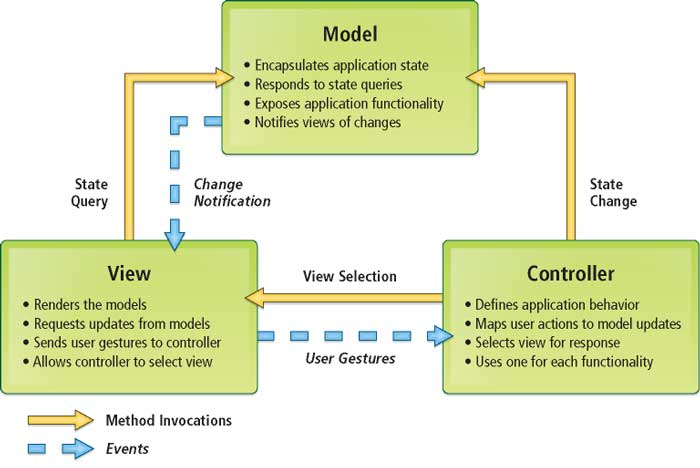
\includegraphics[scale=0.5]{img/mvc}
	\label{fig:mvc}
	\caption{Een voorstelling van de werking van een systeem gebruikmakende van een MVC architectuur}
\end{figure}

\section{Gebruikte technologie}
\label{sec:technologie}
De programmeertaal die gebruikt wordt, is Java. 
In Java wordt gebruik gemaakt van het Spring MVC framework\cite{spring, spring-mvc} voor het ontwikkelen van CalZone. 
De IDE waarin geprogrammeerd wordt, is de meest recente versie van 'Eclipse Classic' met volgende uitbreidingen:

\begin{itemize}
	\item De gehele collectie 'Web, XML, Java EE and OSGi Enterprise Development'	
	\item Spring Tool Suite (uit de Eclipse Marketplace)
	\item De gehele collectie 'Maven Integration for Eclipse'
\end{itemize}
\noindent
Het uitvoeren van de applicatie wordt mogelijk gemaakt door middel van Apache Maven\cite{Maven} en Apache Tomcat\cite{Tomcat}.
De gebruikte databank voor de back-end is MySQL.
De connecties vanuit het logisch niveau van het systeem naar de databank verloopt via Hibernate\cite{hibernate} 
Voor de view wordt gebruik gemaakt van JSP's: een technologie om dynamisch webpagina's te genereren.

	\chapter{Viewpoints}
\label{chap:viewpoints}

In dit hoofdstuk worden \emph{design viewpoints} besproken die relevant zijn voor het systeem. 
\section{Context}
\label{sec:context}

De gebruikers van het systeem zijn onder te verdelen in 5 categorie\"{e}n: externen, studenten, professoren, assistenten en programmabeheerders. 
Het design van CalZone houdt rekening met de functionaliteiten die specifiek aan deze gebruikers zijn toegekend zoals beschreven in het SRS\cite{SRS} van dit project. 
\\

De functionaliteiten die iedere actor in het systeem bezit, worden ge\"{i}llustreerd in de use case diagrammen  \ref{fig:useCaseUsers}, \ref{fig:useCaseAdmin}, \ref{fig:useCaseProf} en \ref{fig:useCaseStudent}.

\begin{figure}[H]
	\centering
	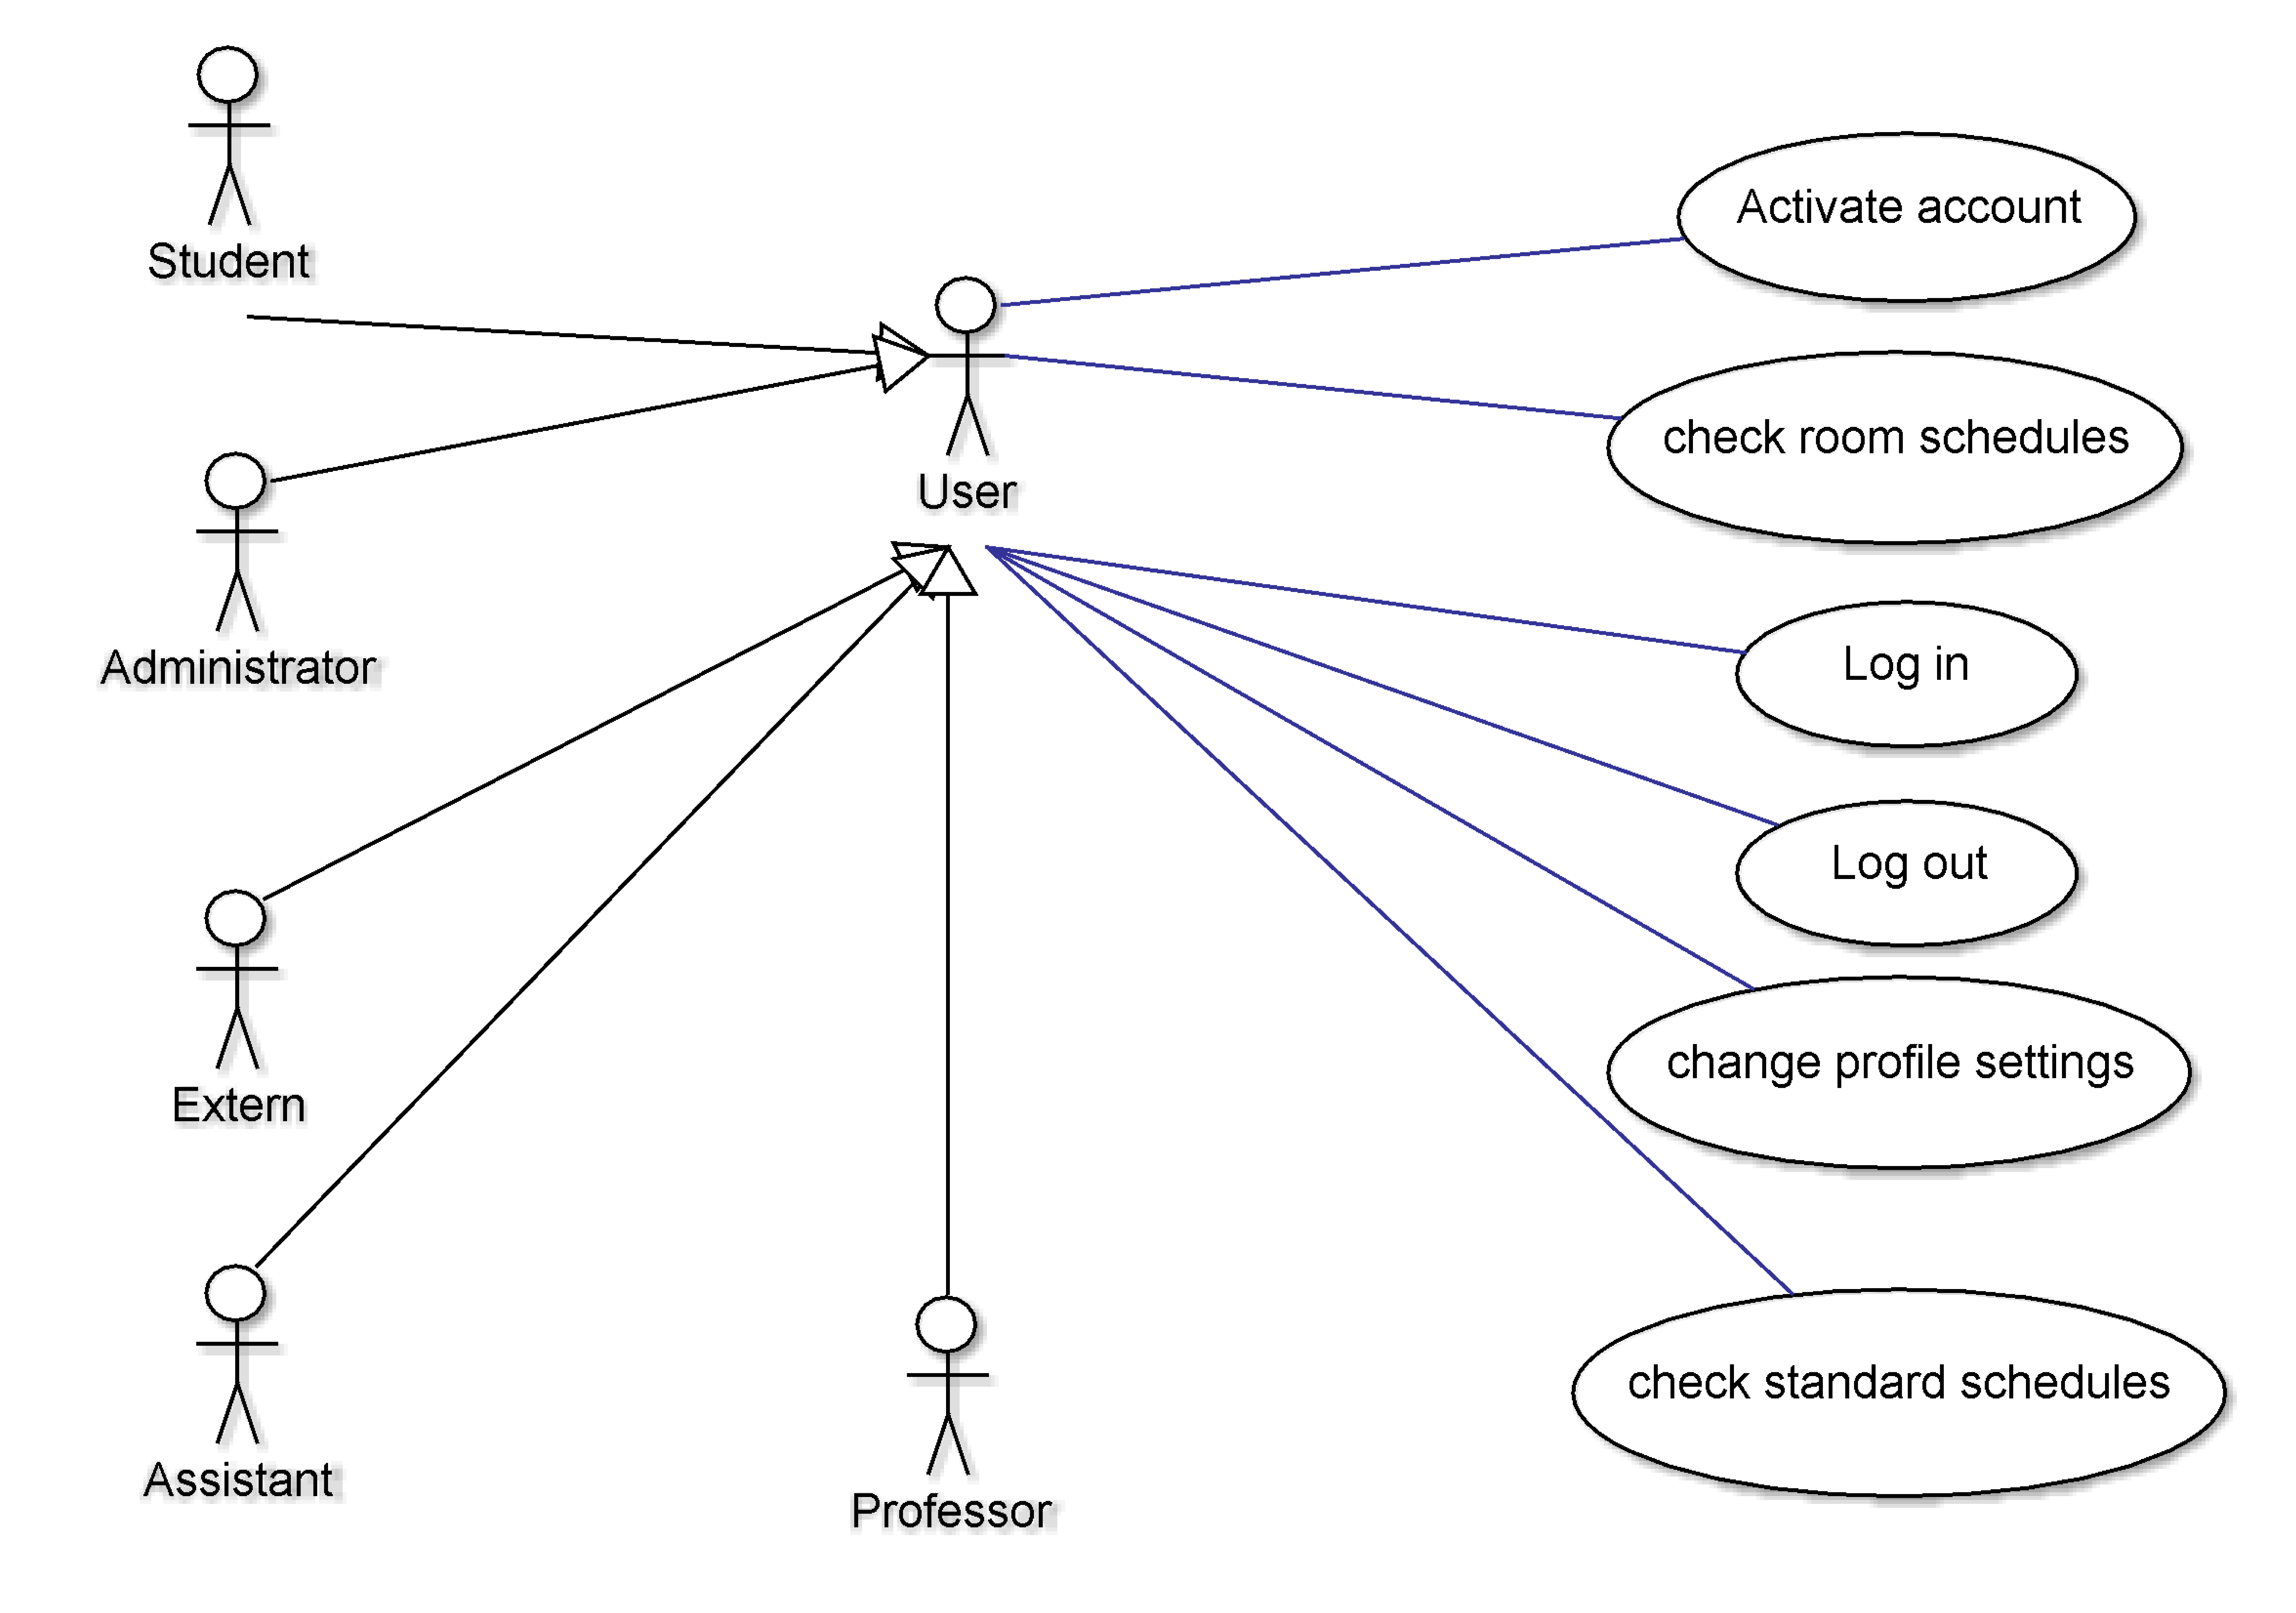
\includegraphics[scale=0.2]{img/useCaseUsers}
	\caption{Use case diagram met focus op de verschillende actoren}
	\label{fig:useCaseUsers}
\end{figure}

\begin{figure}[H]
	\centering
	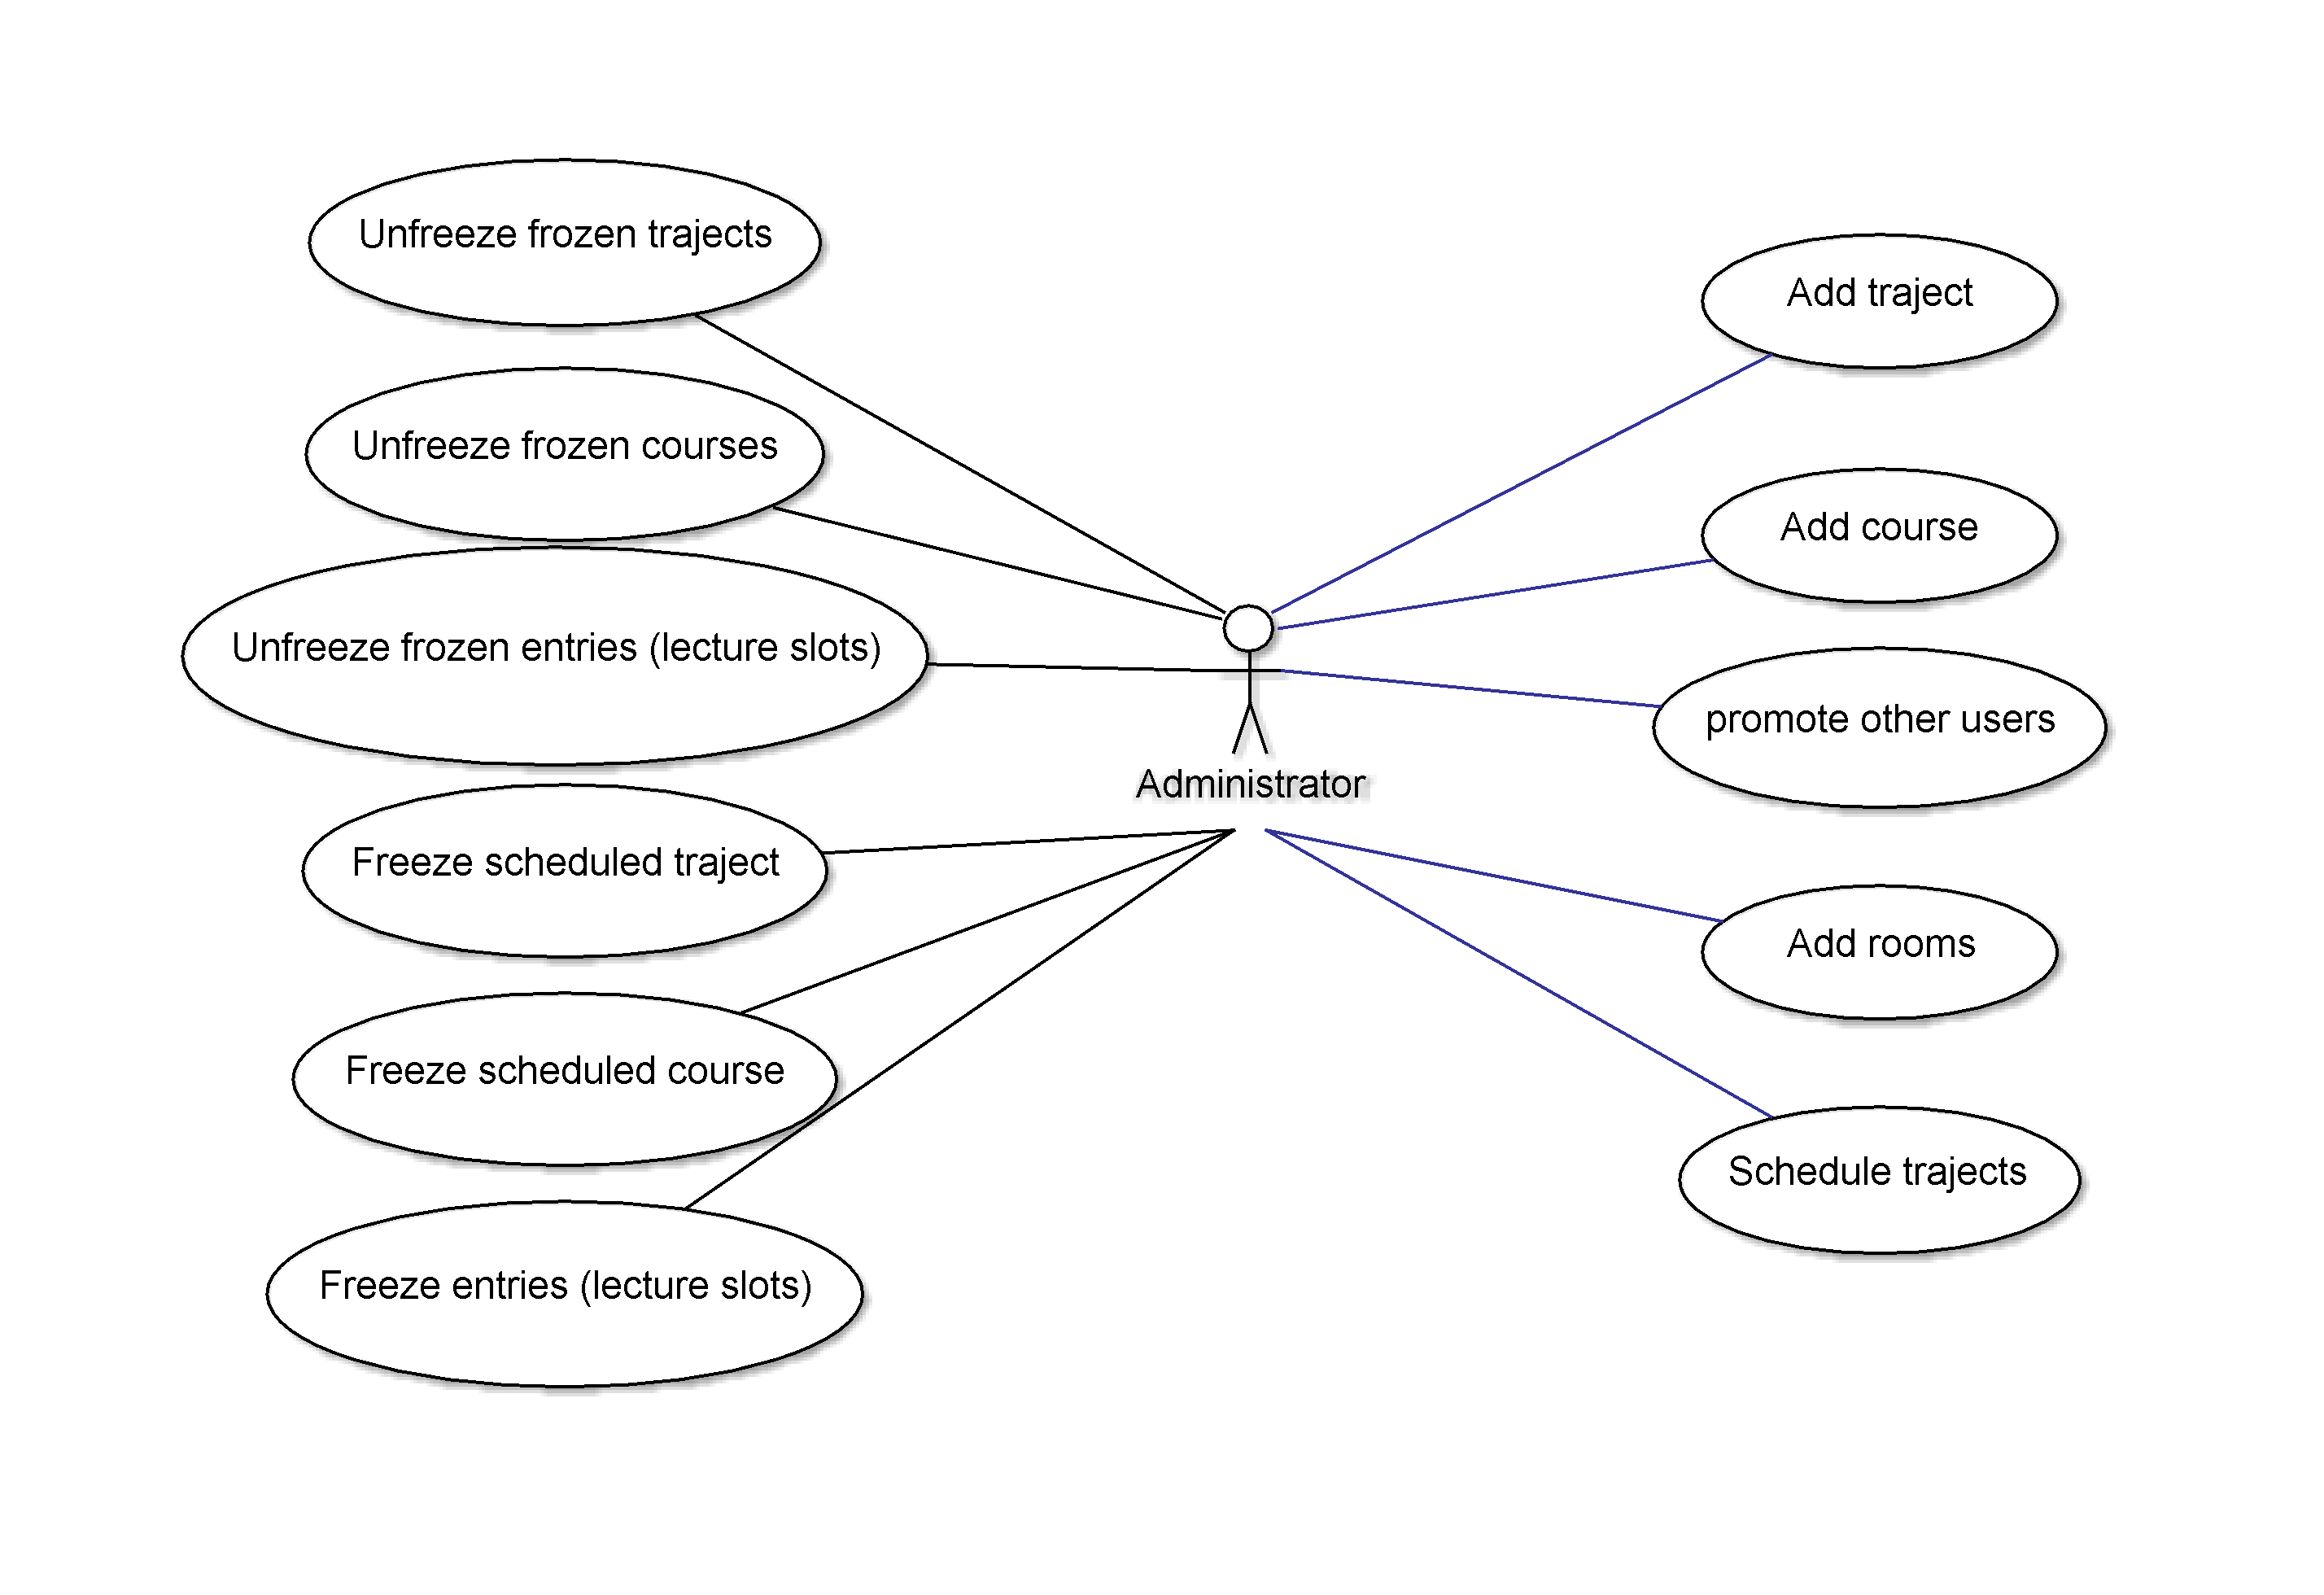
\includegraphics[scale=0.15]{img/useCaseAdmin}
	\caption{Use case diagram met focus op de actor administrator}
	\label{fig:useCaseAdmin}
\end{figure}

\begin{figure}[H]
	\centering
	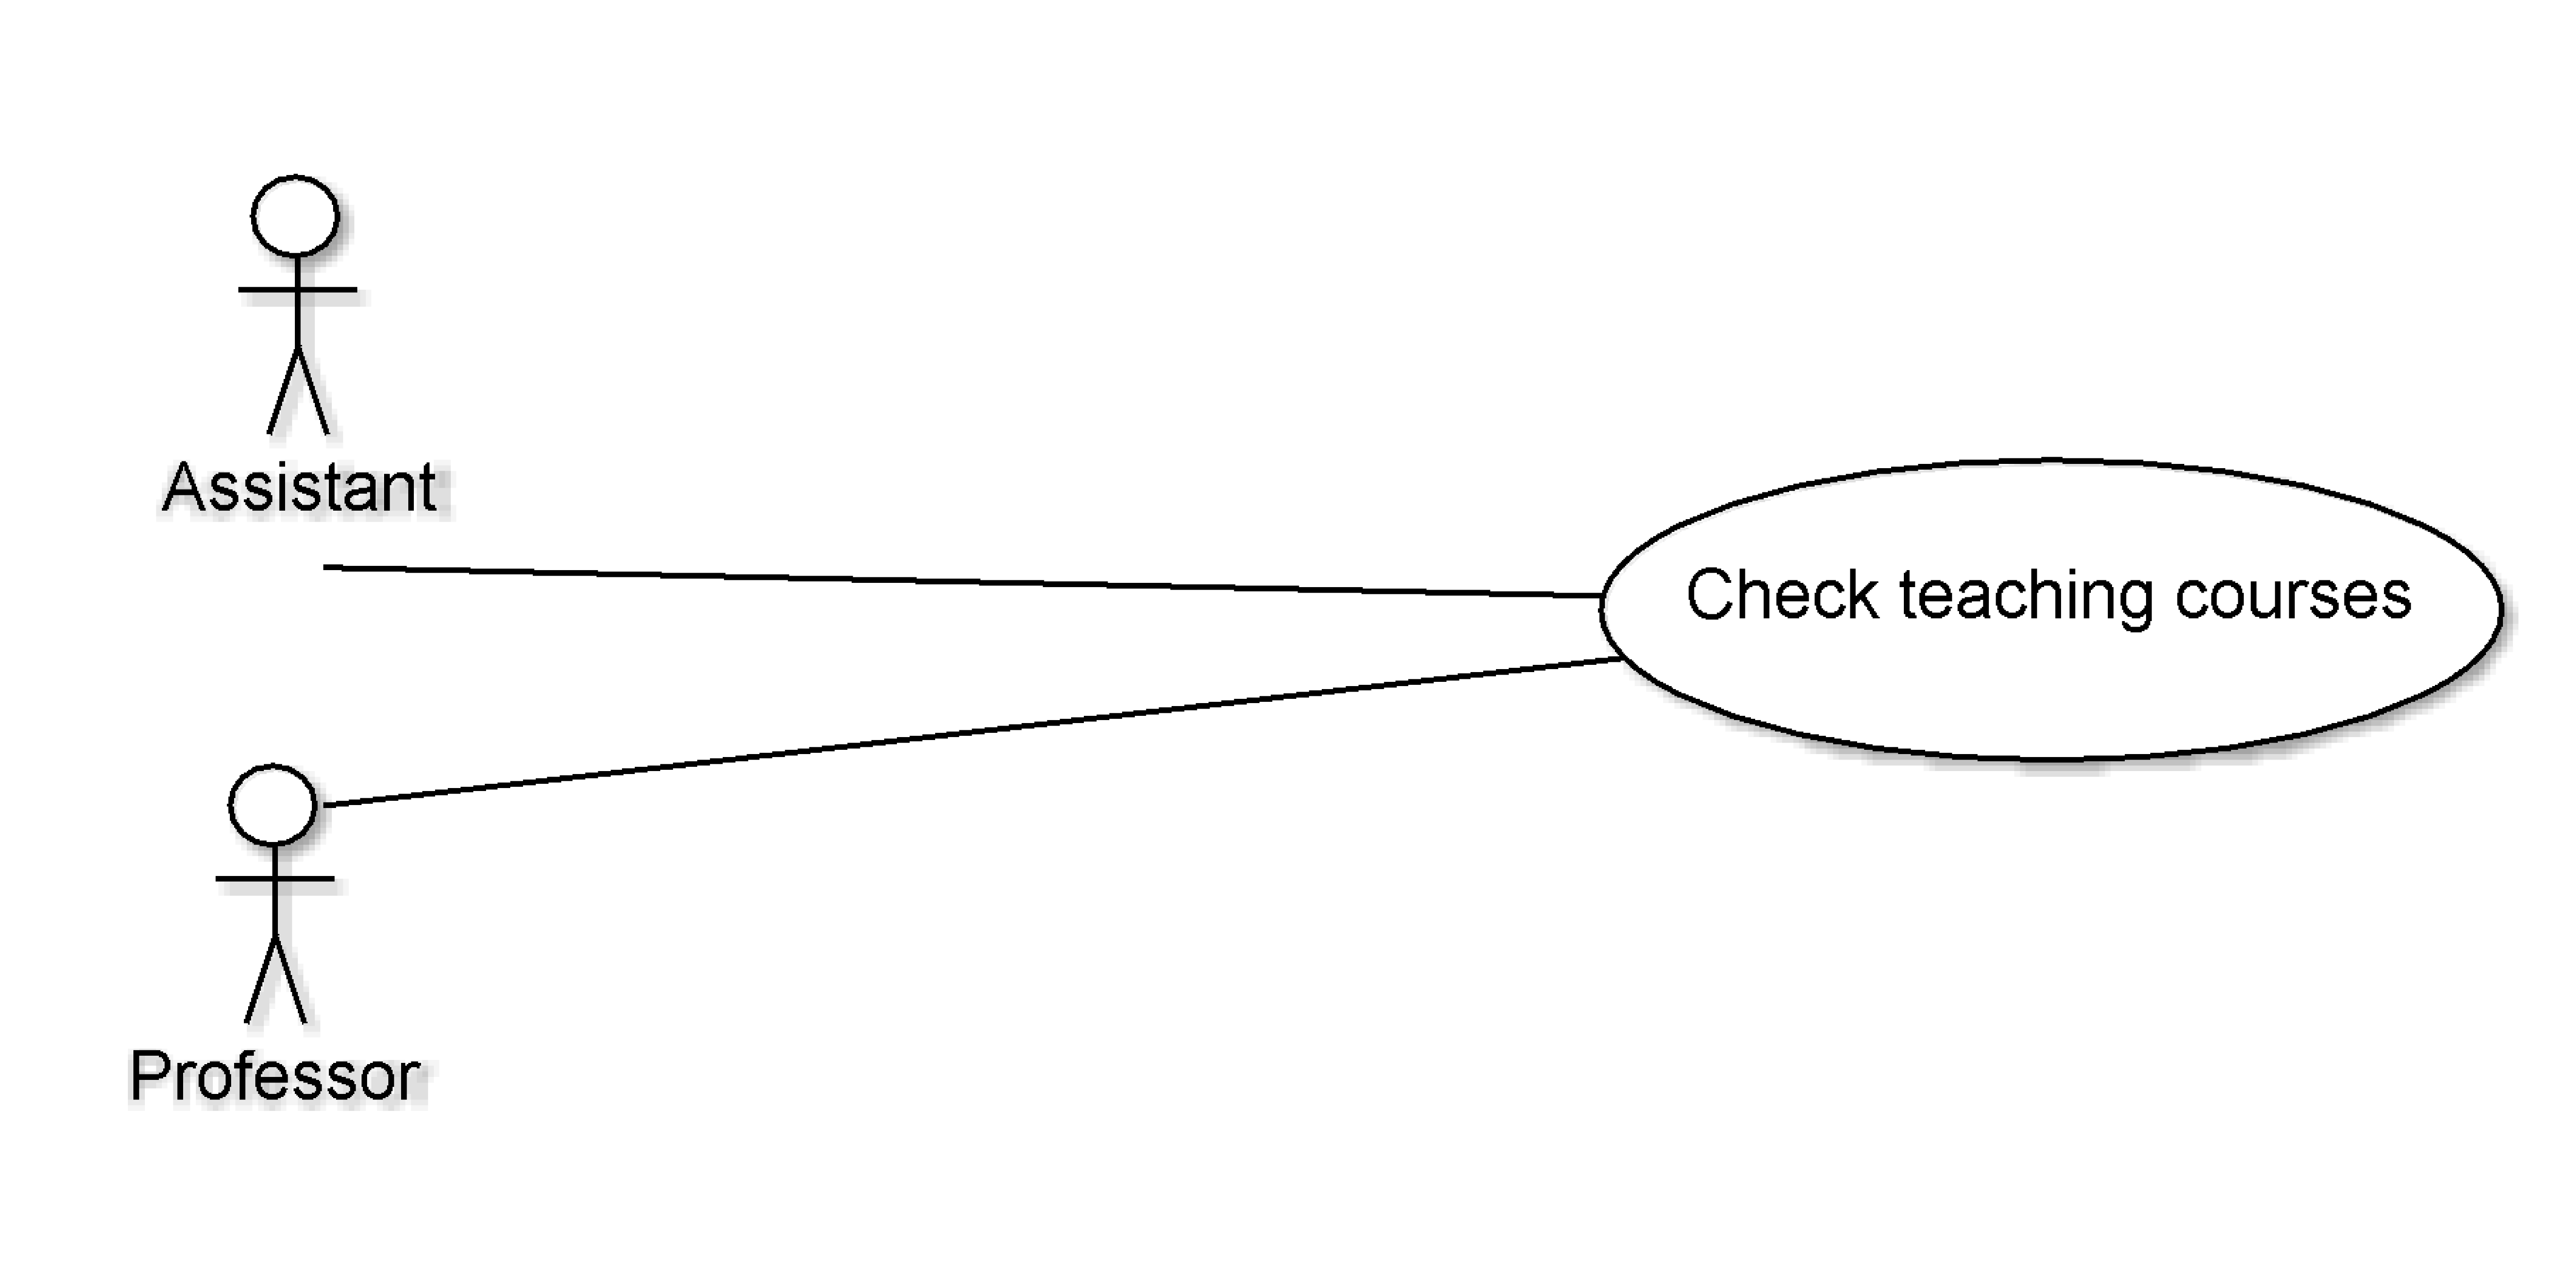
\includegraphics[scale=0.2]{img/useCaseProf}
	\caption{Use case diagram met focus op de actoren professor en assistant}
	\label{fig:useCaseProf}
\end{figure}

\begin{figure}[H]
	\centering
	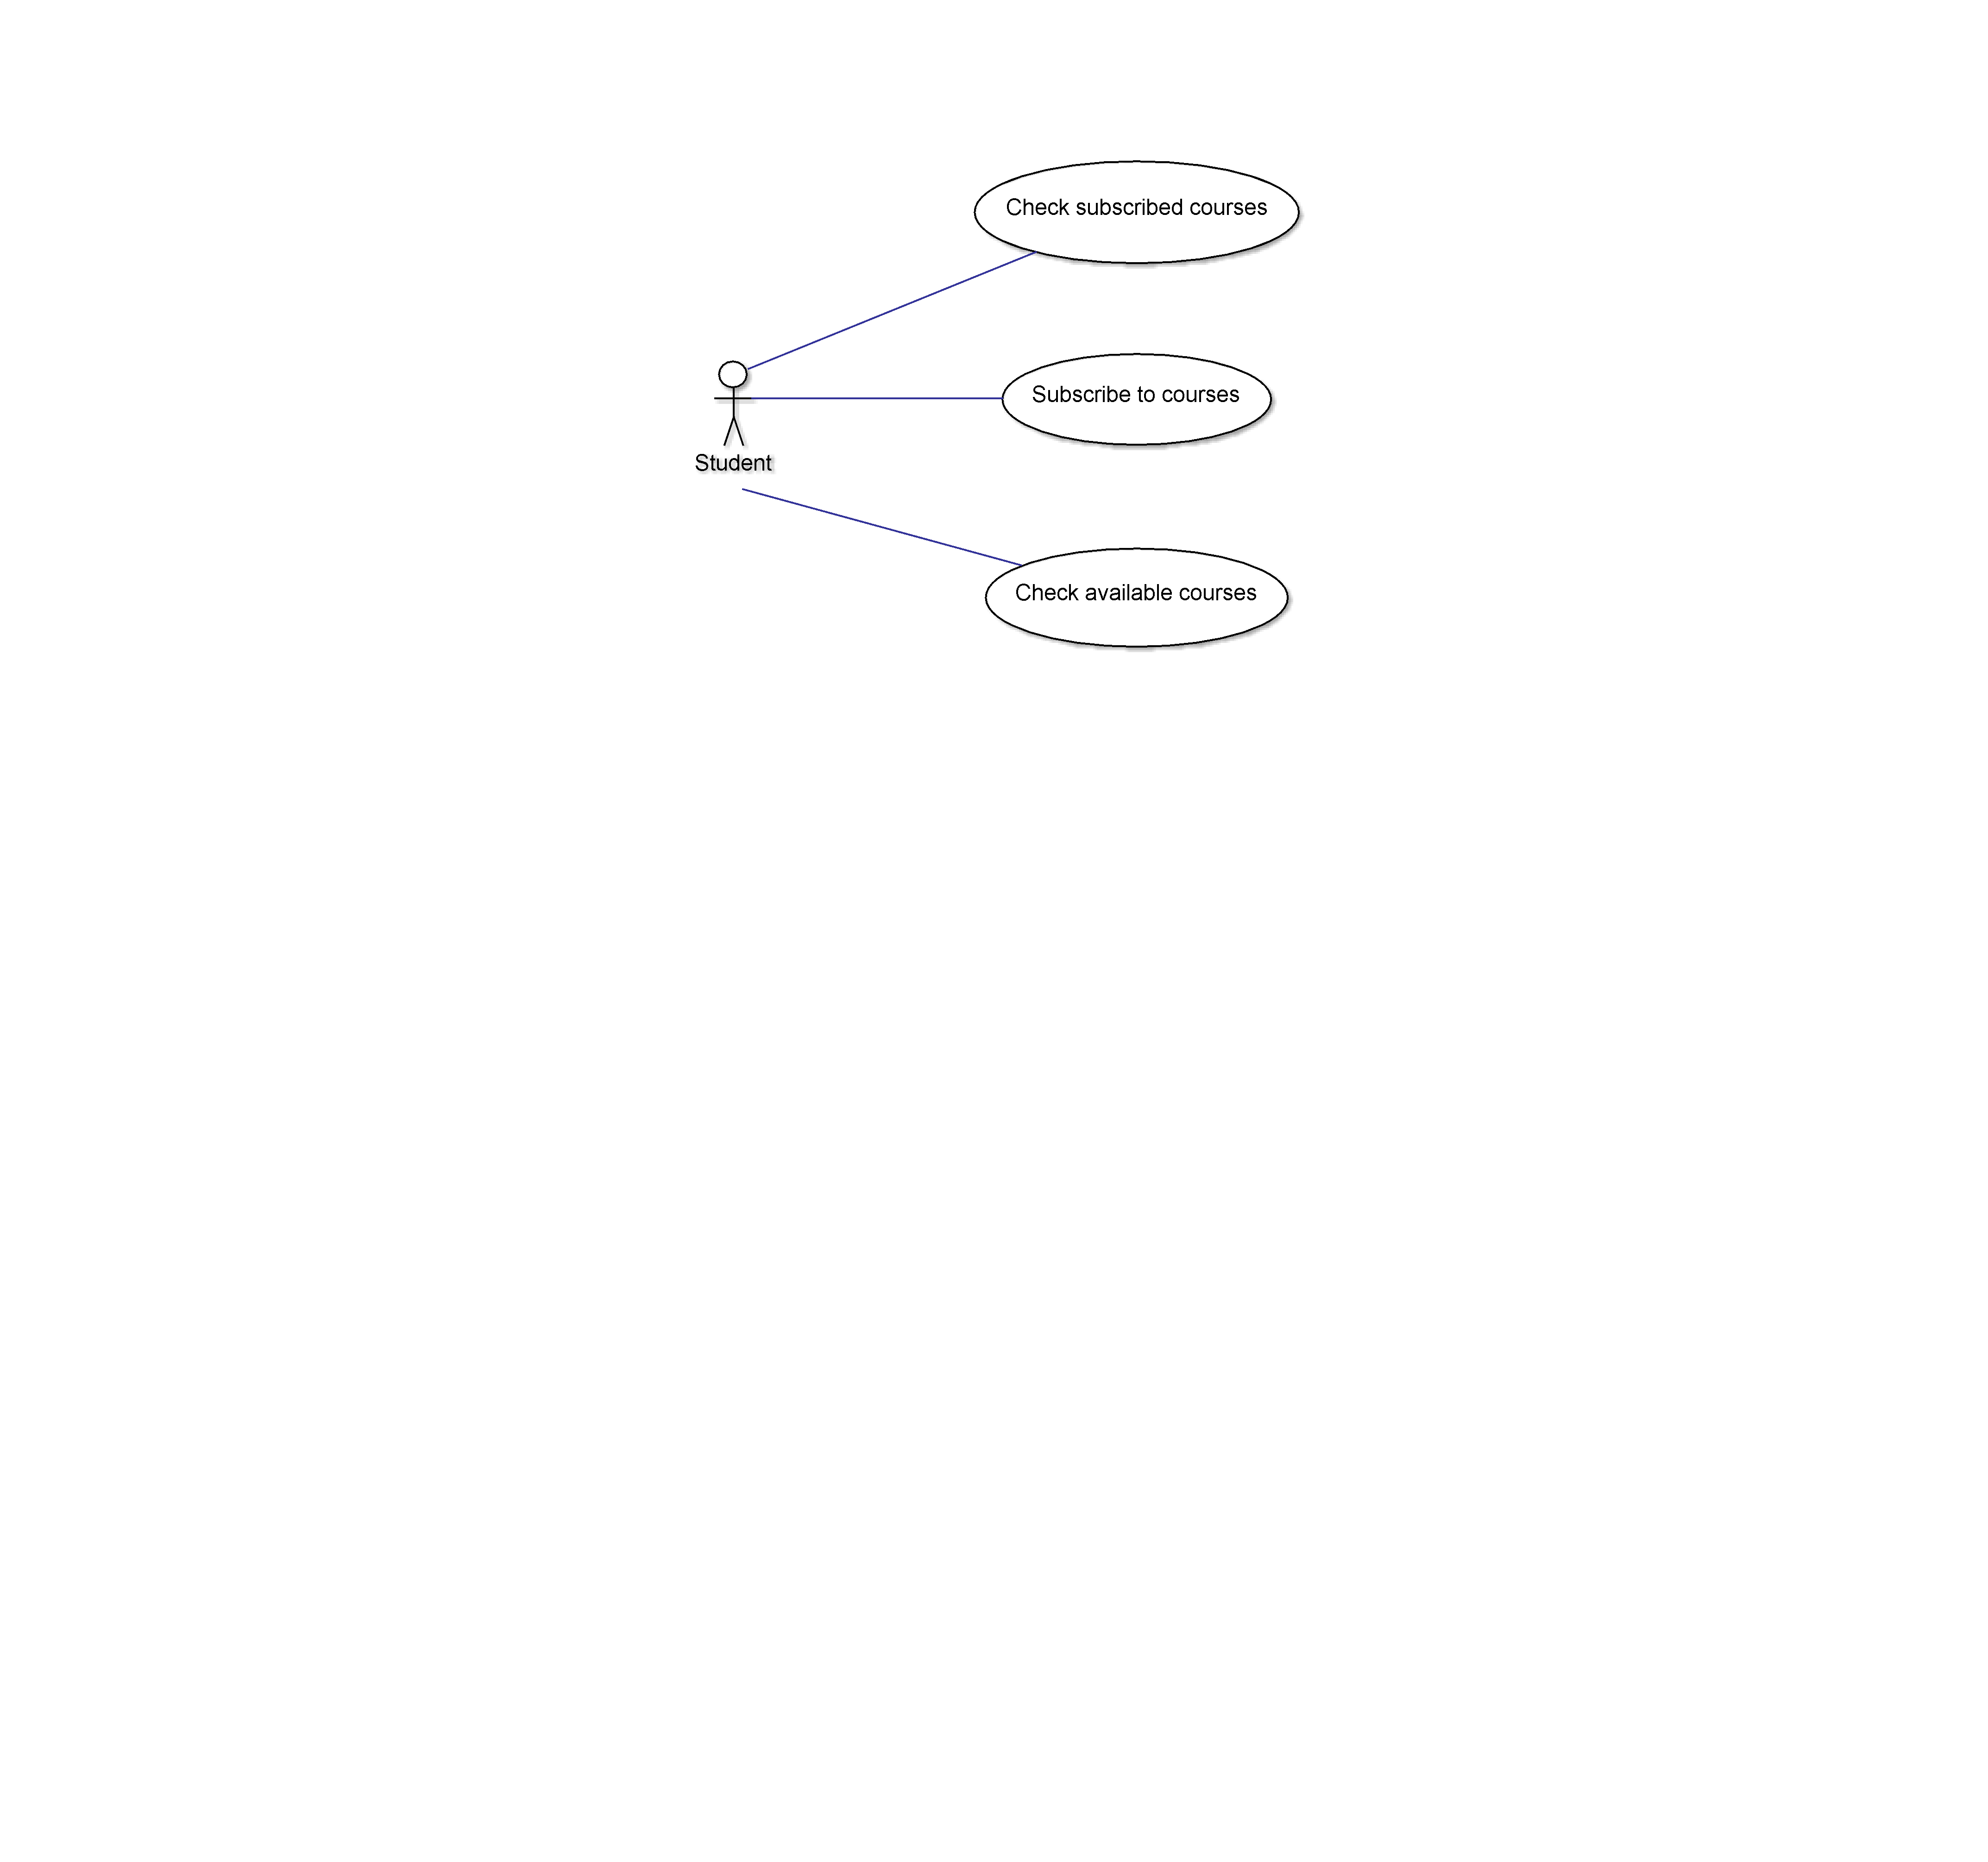
\includegraphics[scale=0.2]{img/useCaseStudent}
	\caption{Use case diagram met focus op de actor student}
	\label{fig:useCaseStudent}
\end{figure}
\section{Logica}
\label{sec:logica}
In deze sectie worden verschillende modules en packages besproken die deel uitmaken van het huidige logische niveau van het systeem.

\subsection{Lagen}
\subsubsection{Database Repositories}
\label{subsubsec:databaseRepo}
CalZone maakt gebruik van een relationele databank, MySQL, als back-end voor dataopslag. 
Om informatie vanuit deze databank te lezen en er naartoe te schrijven zijn er enkele packages voorzien die een abstractie bieden voor het openen en sluiten van de connectie met de databank en het sturen van queries naar de databank.
Dit is de eerste package die bijdraagt tot deze abstractielaag.

\subsubsection{Service}
\label{subsubsec:service}
Dit is de tweede package die abstractie biedt tussen de databank en het logische niveau van het systeem. 
Het abstractieniveau ten opzichte van de data-laag stijgt dankzij deze service-laag.
De klassen in deze package voorzien dus functies om specifieke data vanuit de databank op te halen.
Deze klassen voeren queries uit en laden de gevonden data in de daarvoor voorziene objecten.

\subsubsection{Model}
\label{subsec:model}
Deze package bevat alle klassen die data vanuit de databank bezitten. De klassen in deze package representeren dus de informatie waarmee het systeem functionaliteiten zal voorzien naar de gebruiker toe.

\subsection{Componenten}
\subsubsection{Controllers}
\label{subsubsec:controllers}
Deze klassen zijn verantwoordelijk om de HTTP-requests te verwerken. 
Deze klassen zorgen dus voor een propagatie van (functionaliteits)verzoeken van de front-end naar de back-end. 
Eveneens zorgen deze klassen ook voor een propagatie van data van de back-end naar de front-end. 
Dit laatste uit zich in content op de webpagina's.
Met andere woorden zorgen de controllers dus voor de mogelijke views en voorzien dus de mogelijkheid om de functionaliteiten opgesomd in de use case diagrammen van sectie~\ref{sec:context} uit te voeren. 

\subsubsection{Validators}
\label{subsec:validators}
Binnenin het systeem dient sommige data gecontroleerd te worden op geldigheid. 
Deze validatorklassen zijn verantwoordelijk om geldigheid van bepaalde informatie te controleren en aan te geven indien deze info niet geldig is.

\subsubsection{Scheduler}
\label{subsec:scheduler}
In deze package zitten de klassen die bijdragen tot het maken en formuleren van lessenroosters.
Ook vind je hier de configuraties voor OptaPlanner.
Er is een configuratiebestand voor de uiteindelijke AI agent die lessenroosters zal trachten te maken op basis van verschillende constraints.
OptaPlanner bezit een benchmarking systeem opdat men verschillende configuraties kan testen op verscheidene datasets.
Meer hierover is te vinden in het Test Document van dit project.
Deze package bezit ook een file met constraint regels.
Deze file bevat code in de programmeertaal Drools\cite{Drools}.

\subsubsection{Exception}
\label{subsec:exception}
Zelfgemaakte Exceptions worden verzameld in deze package.
\section{Data}
\label{sec:data}
De evolutie die het design in deze iteratie heeft ondervonden is vooral te merken in de database.
Het datamodel is uitgebreid opdat de databank in staat is om vakken, lokalen en allerhande concepten omtrend deze vakken en lokalen op te kunnen slaan. Deze concepten zullen laterinvloed hebben op het plannen van de lessenroosters en lokalenroosters via de scheduler.\\

Ook werden aanpassingen uitgevoerd aan het user management zodat bij implementatie gebruik gemaakt kon worden van de module Spring Security\cite{spring-security} om de authenticatie van gebruikers af te handelen.\\

Figuur~\ref{fig:EER diagram} toont het EER-model van de databank. Om overzicht te bewaren worden de attributen die iedere entiteit bezit niet weergegeven in dit model.

\begin{figure}[H]
	\centering
	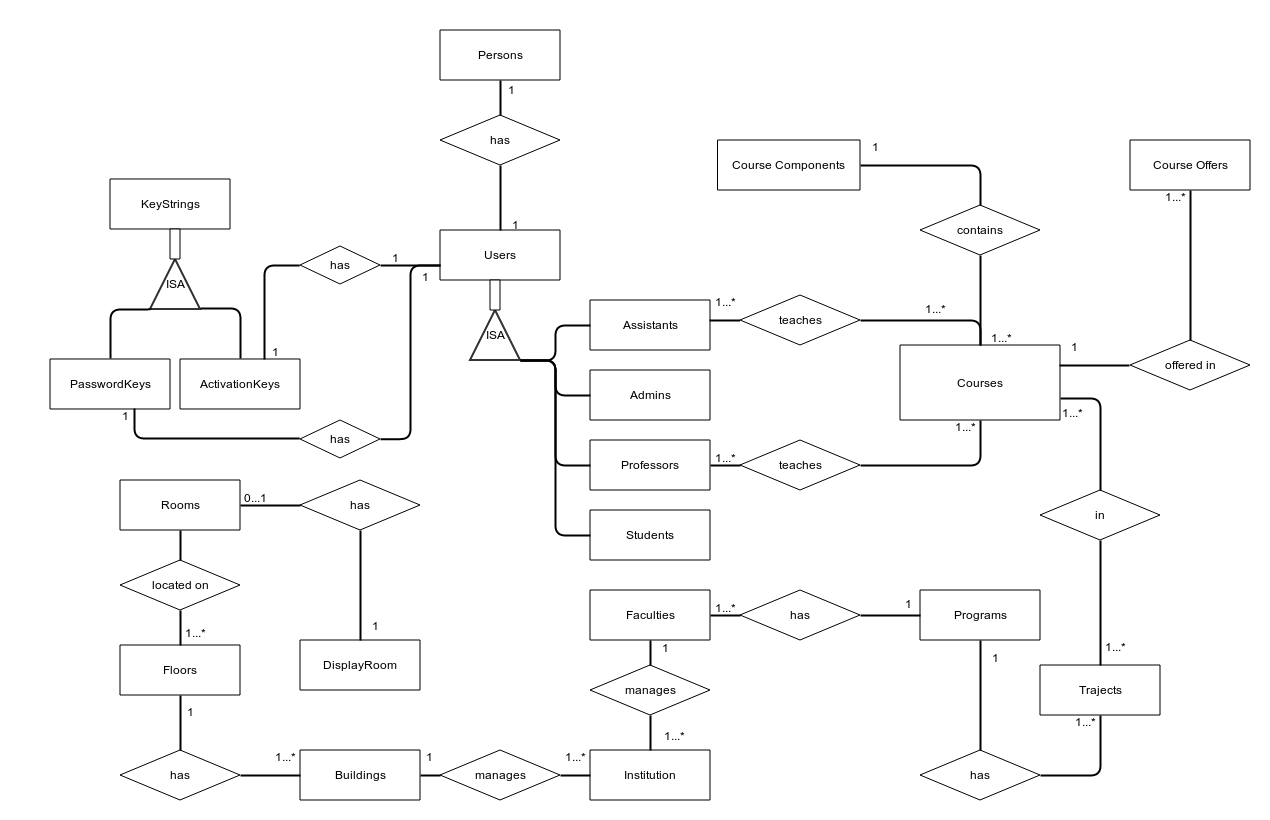
\includegraphics[scale=0.4]{img/ER2-gliffy}
	\caption{EER diagram}
	\label{fig:EER diagram}
\end{figure}

\section{Structuur}
Deze sectie beschrijft de structuur van belangrijke en interessante onderdelen van het systeem. 
Deze beschrijvingen worden al dan niet ondersteund met een bijbehorend diagram indien dit van toepassing is.

\subsection{Leslokalen en vakken}
Volgend UML diagram beschrijft de structuur van de verscheidene klassen betreffende leslokalen en lessen die met elkaar gerelateerd zijn op het logisch niveau van het systeem.
Deze klassen bezitten data vanuit de databank die nodig zullen zijn om lessenroosters en examenroosters te plannen.

\begin{figure}[H]
	\centering
	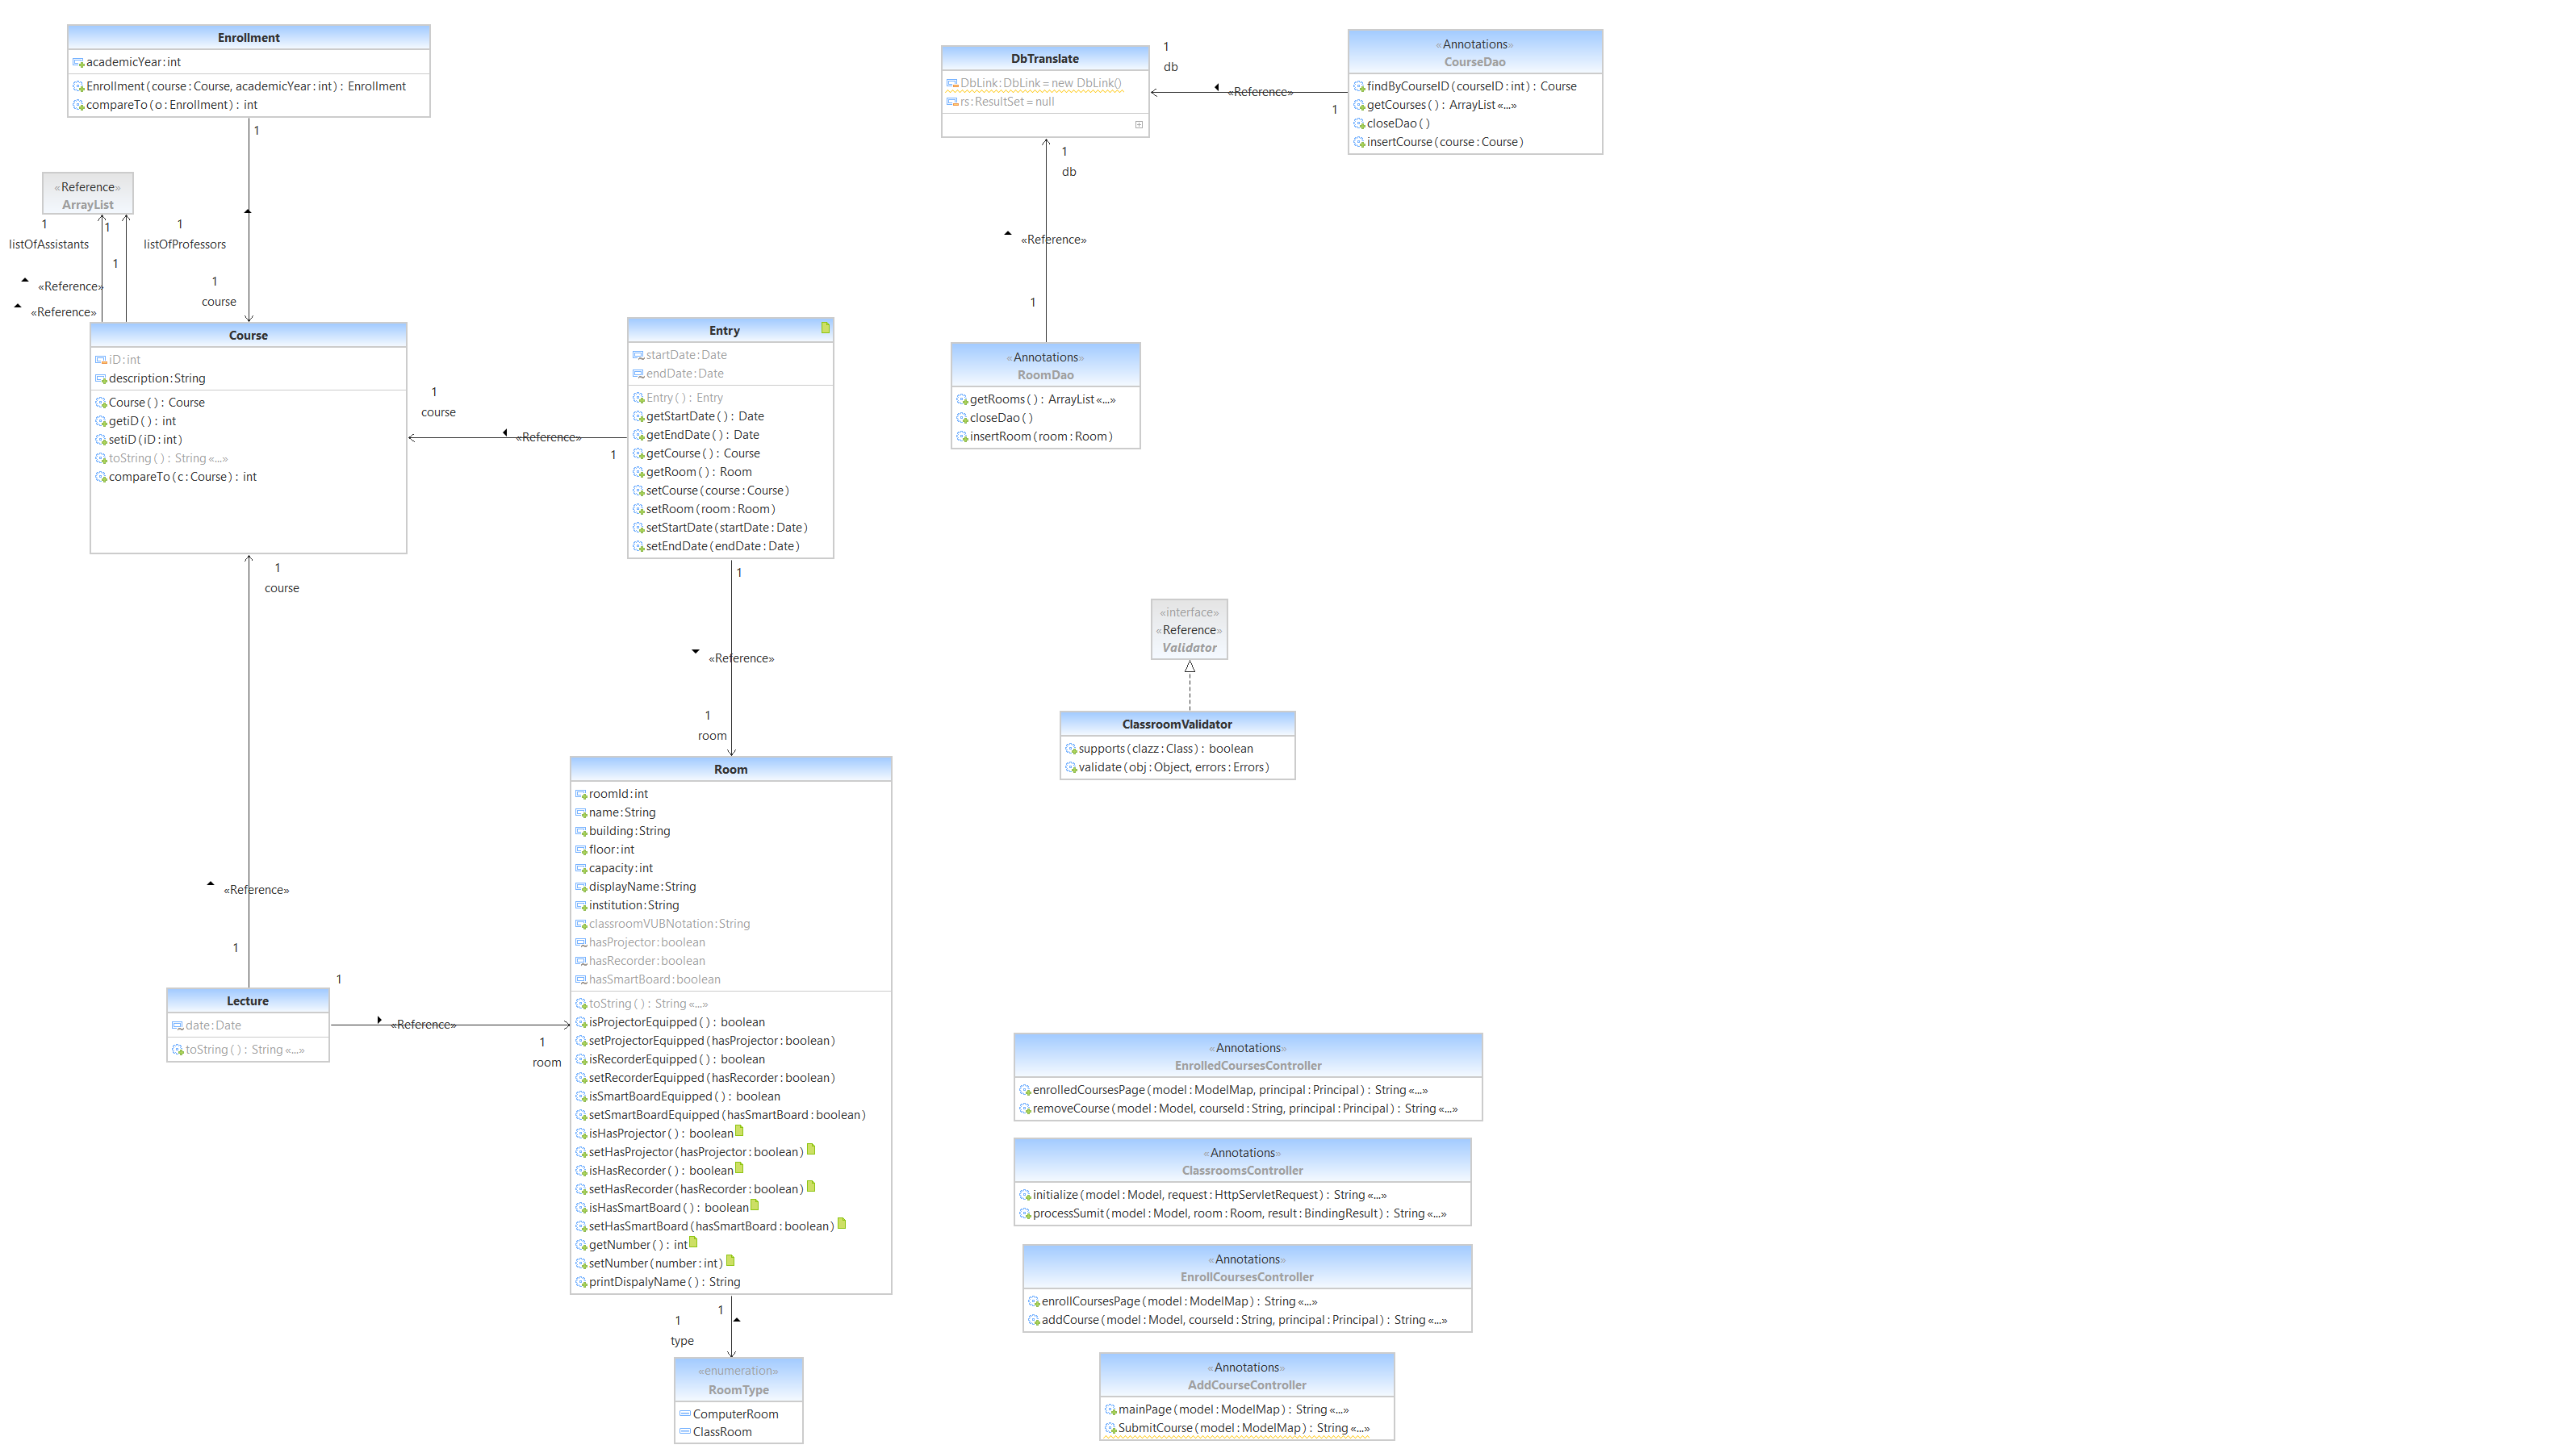
\includegraphics[scale=0.4]{img/roomsAndCourses}
	\caption{UML klassediagram voor leslokalen en vakken}
	\label{fig:roomsAndCourses}
\end{figure}

\subsection{Logging}
\label{subsec:logging}
Als logging framework werd gekozen voor SLF4J\cite{slf4j}.
Dit framework is echter een API die het maken van logs versimpelt voor de programmeur en vereist dus nog een geconfigureerde backbone.
Als backbone werd gekozen voor logback \cite{logback}.\\

In loggingsystemen kan men verschillende soorten logberichten produceren. 
Het systeem zorgt er dan voor dat deze berichten op de juiste plaats terecht komen.
De belangrijkste soorten berichten zijn: info, warning, error en debug.
In wat volgt wordt de configuratie van het loggingsysteem uitgeklaard.\\

Alle logberichten worden op de standaard output getoond.
Verder worden er specifieke logs opgeslagen naar bestanden.
Er zijn 2 folders voorzien voor logs: eentje voor debug logs en een folder met daarin een algemene log file.
Deze algemene log file bevat log berichten vanaf het niveau 'INFO', wat betekent dat het dus INFO, WARNING en ERROR logs bewaart.
Voor de debug logs wordt iedere dag een nieuwe file aangemaakt omdat het systeem een massa aan debug logs kan produceren op een dag.\\

Voor het in productie gaan van de applicatie is het sterk aangeraden de debug logs uit te schakelen om de lengte van de totale hoeveelheid logs drastisch te krimpen.

\subsection{Scheduler}
\subsubsection{Scheduling}
\label{subsec:scheduleclass}
Volgend UML klassediagram beschrijft de structuur van de klassen betreffende lessenroosters en het maken van zulke roosters.
Figuur \ref{fig:scheduling} beschrijft hoe het planningsprobleem in onze applicatie geformuleerd wordt.
Het framework OptaPlanner\cite{optaplanner} maakt gebruik van deze klassen door middel van annotaties om lessenroosters te maken.
Nu volgt een simpele beschrijving van de structuur.\\

Een \textit{Schedule} is een planning.
Zo een planning bestaat uit een sequentie van \textit{Entries}.
Een \textit{Entry} kan men vergelijken met een afspraak in een agenda.
In ons systeem wordt zo dus gevormd door een klaslokaal (Room), een vakonderdeel (CourseComponent) en een tijdstip (Date).
Een initialisatieklasse, \textit{SchedulerInitializer}, voorziet de beschikbare datums en tijdstippen.
Het verwezenlijken van een planning wordt opgelost door de klasse \textit{SchedulerSolver}.
Deze klasse zal gebruik maken van OptaPlanner om een \textit{ Schedule} te genereren.
Impliciet zal de \emph{SchedulerSolver} gebruik maken van de klassen \emph{SchedulerHelper}, \emph{EntryDifficultyComparator}, \emph{RoomStrengthComparator}, \emph{DateStrengthComparator} in een poging een zo goed mogelijk lessenrooster te bekomen.
De klasse \emph{MovableSelectionEntry} zorgt ervoor dat OptaPlanner weet welke entries verschoven mogen worden door de solver en welke niet.
Er is dus een notie van bevriezen van entries aanwezig in de schedule.
Meer uitleg over hoe OptaPlanner werkt en geconfigureerd is wordt beschreven in \ref{subsec:scheduling}.\\

De klasse \emph{SchedulerSolver} is een subtype van de klasse \emph{SchedulerScoreCalculator}.
Deze klasse is verantwoordelijk het berekenen van de score van een \emph{Schedule} in zijn huidige staat.
Via deze klasse kan men ook conflicten gaan detecteren.


Alle klassen in het klassenmodel, op de klasse \emph{HardSoftLongScore} na, diende zelf geschreven te worden en geannoteerd te worden zodat OptaPlanner deze klassen kon herkennen en gebruiken.
Bij het maken van deze klassen diende bepaalde interfaces van OptaPlanner ge\"{i}mplementeerd te worden, Solution\footnote{\url{https://docs.jboss.org/drools/release/6.0.1.Final/optaplanner-javadoc/org/optaplanner/core/impl/solution/Solution.html}} en ScoreDirector\footnote{\url{https://docs.jboss.org/drools/release/6.0.1.Final/optaplanner-javadoc/org/optaplanner/core/impl/score/director/ScoreDirector.html}} en werd de klasse HardSoftLongScore gebruikt.
In het klassediagram werden deze aangeduid met de annotatie \emph{$\langle\langle OPTAPLANNER\rangle\rangle$}.\\


\begin{landscape}
	\begin{figure}[H]
		\centering
		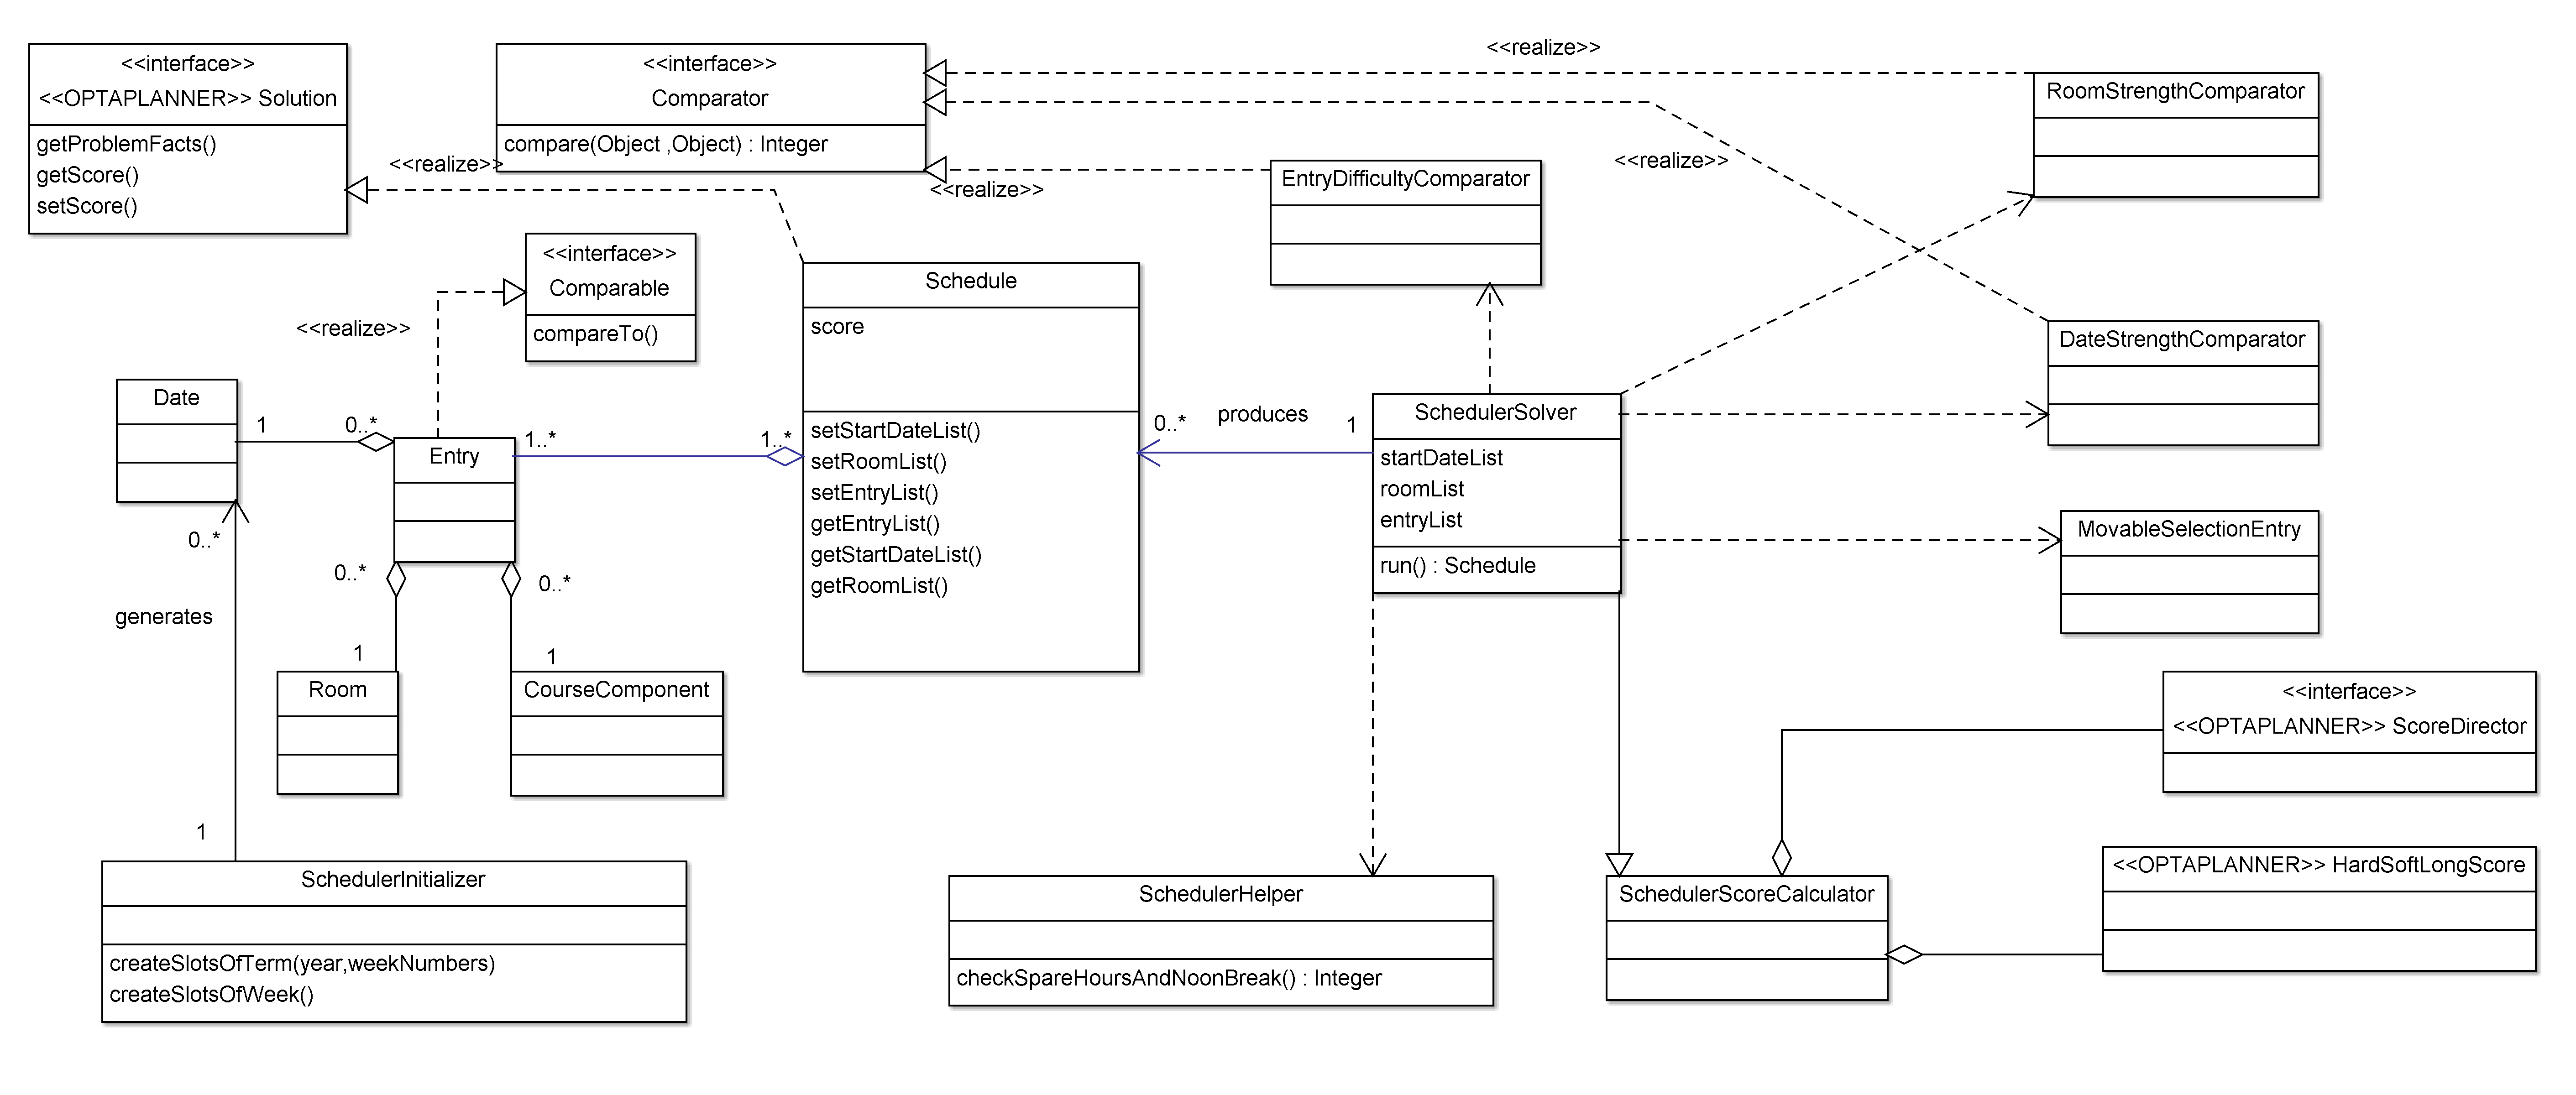
\includegraphics[scale=0.125]{img/scheduler}
		\caption{UML klassediagram voor scheduling}
		\label{fig:scheduling}
	\end{figure}
\end{landscape}

\subsubsection{Conflictdetectie in roosters}
\label{subsubsec:conflicts}
De interface \emph{ScoreDirector}\footnotemark[\value{footnote}] van OptaPlanner is verantwoordelijk om de score van de staat van een planningoplossing te berekenen.
Naast het berekenen van deze score, is de klasse ook in staat om te verklaren hoe hij aan die score komt. 
De \emph{ScoreDirector} voorziet een \emph{justificationList}, een lineaire structuur die informatie bevat over welke regels uit de Drools file afgevuurd zijn.
Aangezien deze regels declaratief zijn en er dus gebruik wordt gemaakt van pattern matching, staat er ook in de \emph{justificationList} welk patroon (de verzameling objecten die voldoet aan de match) er gevonden werd.\\

Dit stelt ons in staat deze informatie te parsen en te vertalen naar ons eigen design om conflicten in een schedule te melden aan de programmabeheerders en professoren die gebruik maken van CalZone.
Figuren \ref{fig:conflictdetection} en \ref{fig:constraintviolations} beschrijven de structuur van de objecten die dit tot stand brengen.\\

Een klasse \emph{ConstraintChecker} zal de \emph{justificationList} van de \emph{ScoreDirector} van OptaPlanner analyseren en een lijst van schendingen teruggeven.
Zo een schending wordt voorgesteld door de interface \emph{ConstraintViolation}.
Deze interface bezit een methode 'description'.
Deze methode geeft een string terug die het gehele conflict uitlegt.
De klasse \emph{ConstraintChecker} is dus het aanspreektpunt voor de front-end om conflicten in een bestaand rooster weer te geven aan gebruikers.\\

Voor iedere constraint is er een klasse voorzien die de interface \emph{ConstraintViolation} implementeert en dus een beschrijving ontwikkelt afhankelijk van wat voor constraint geschonden werd.\\

Het genereren van deze klasses voor de \emph{ConstraintChecker} wordt afgehandeld door een andere klasse: \emph{ConstraintViolationFactory}.

\begin{figure}[H]
	\centering
	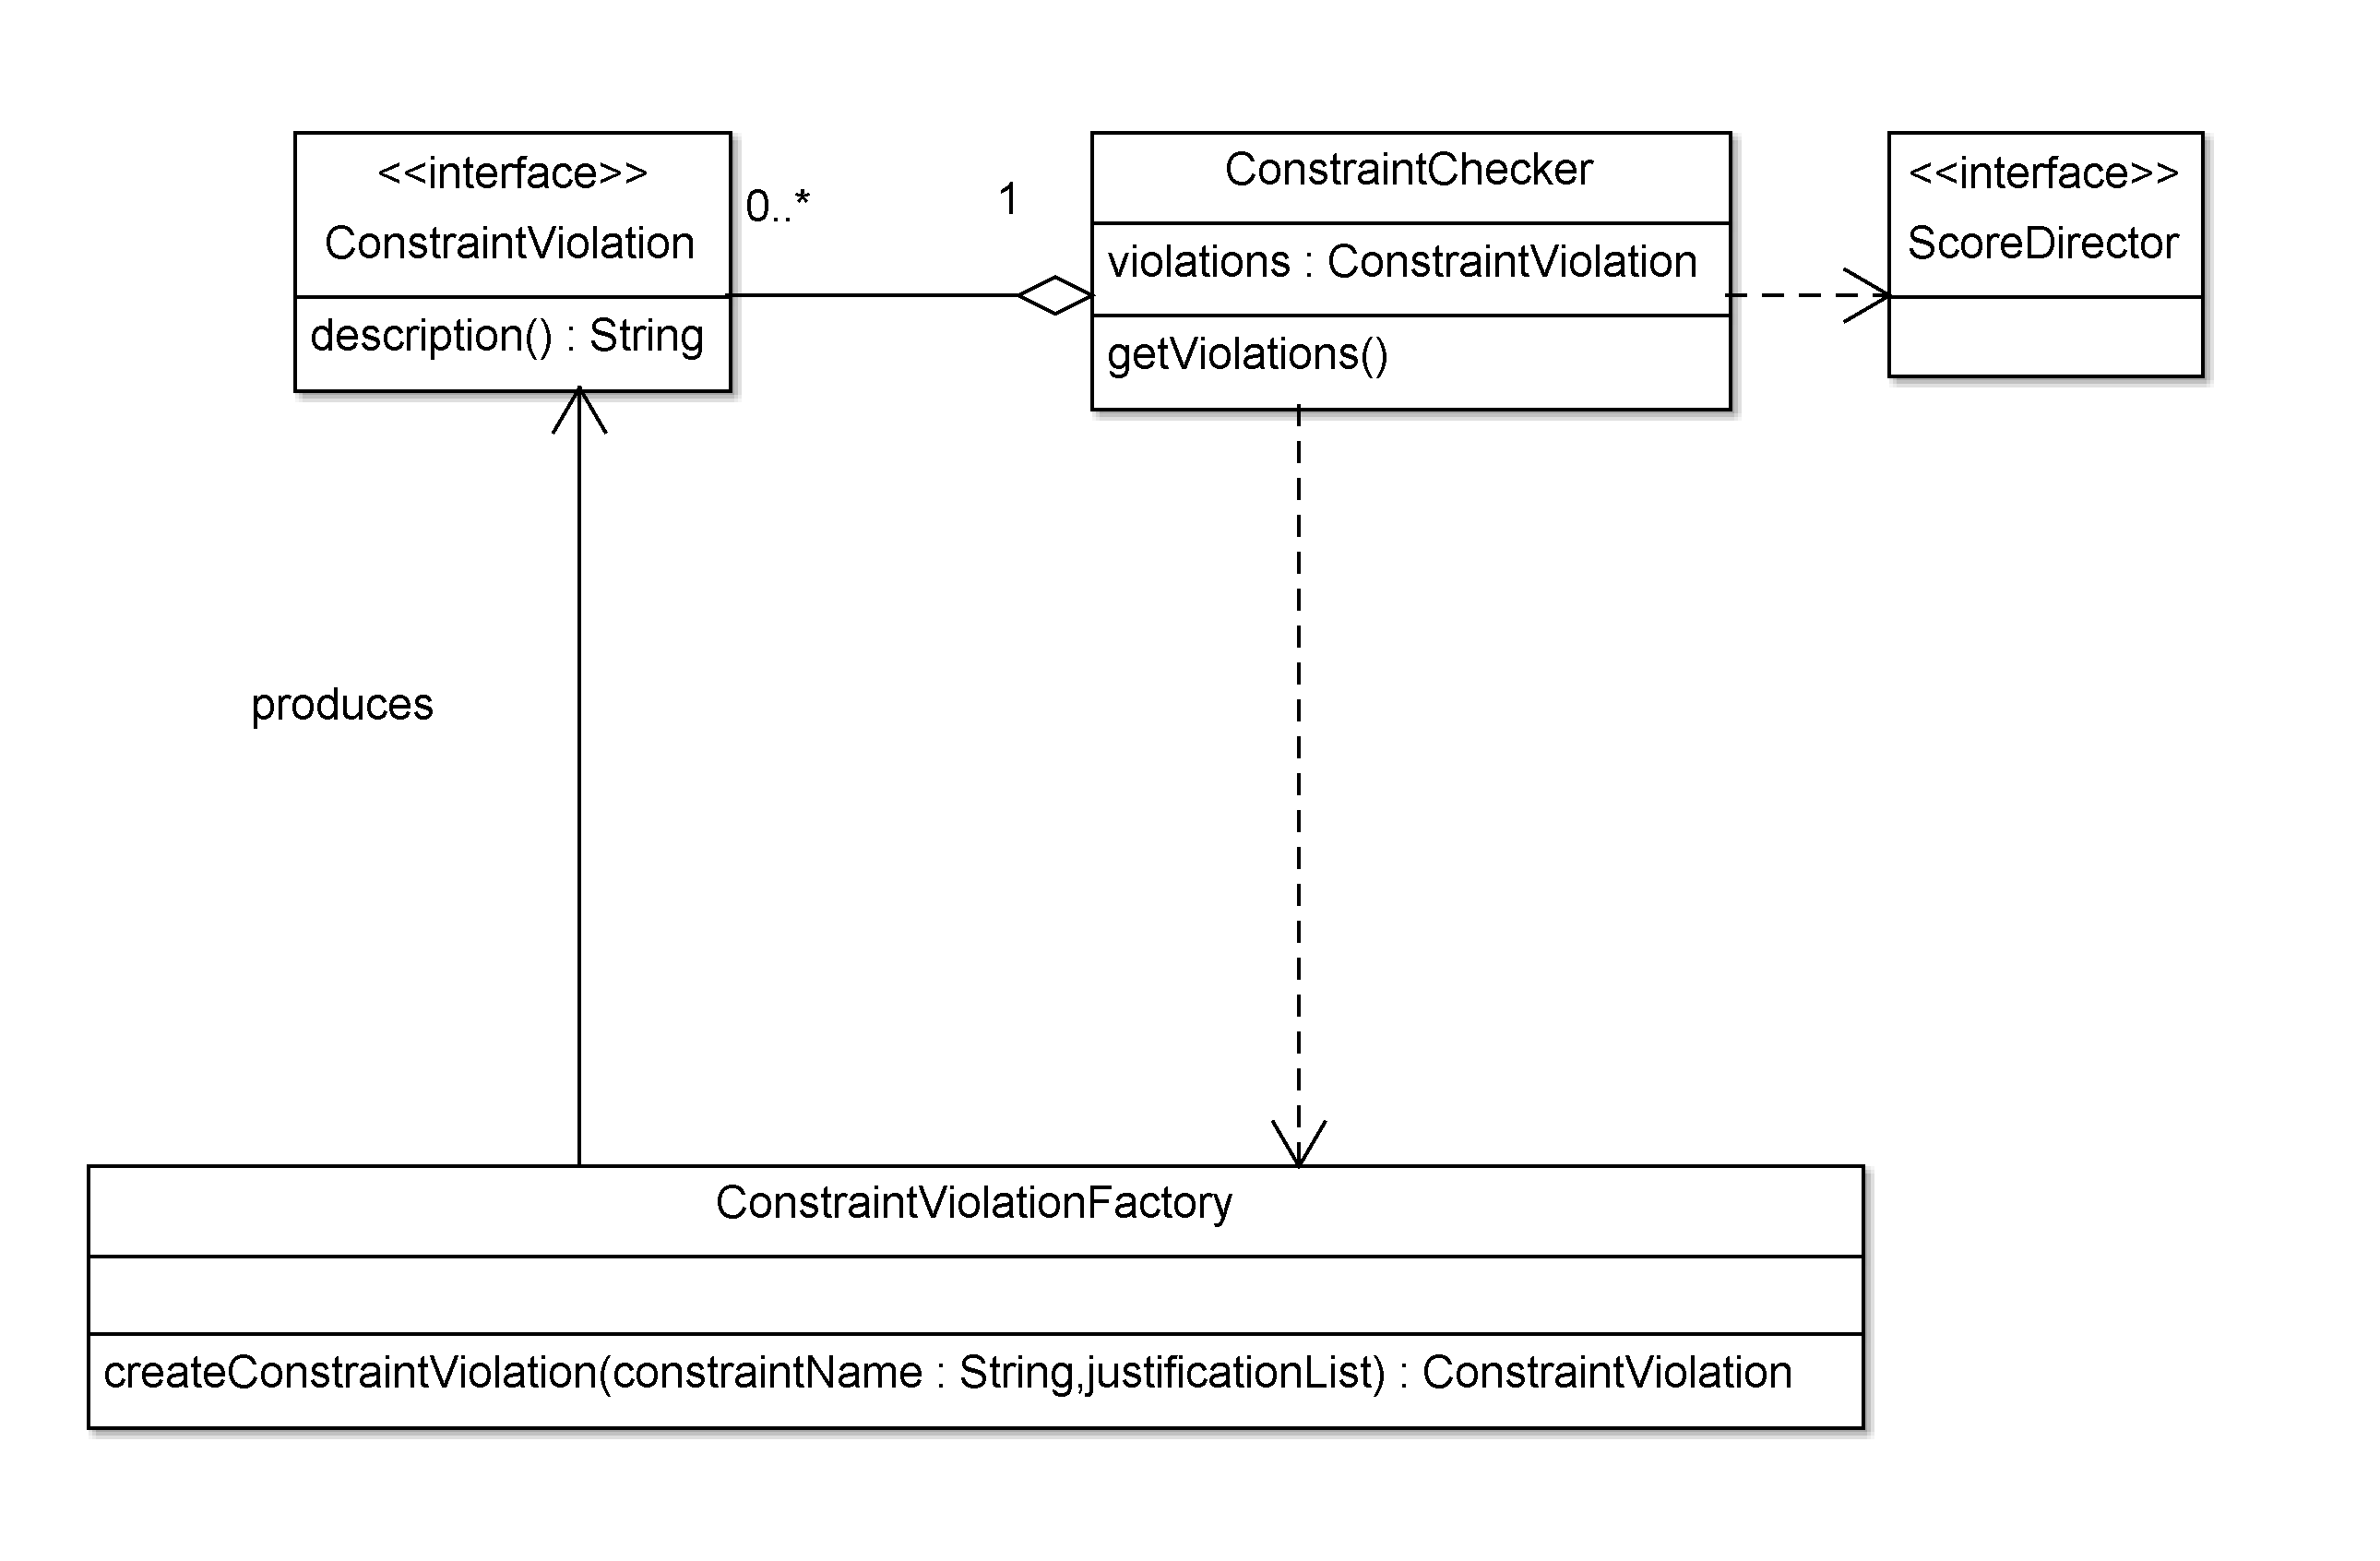
\includegraphics[scale=0.15]{img/conflictdetection}
	\caption{UML klassediagram voor conflictdetectie te realiseren}
	\label{fig:conflictdetection}
\end{figure}

 
\begin{figure}[H]
	\centering
	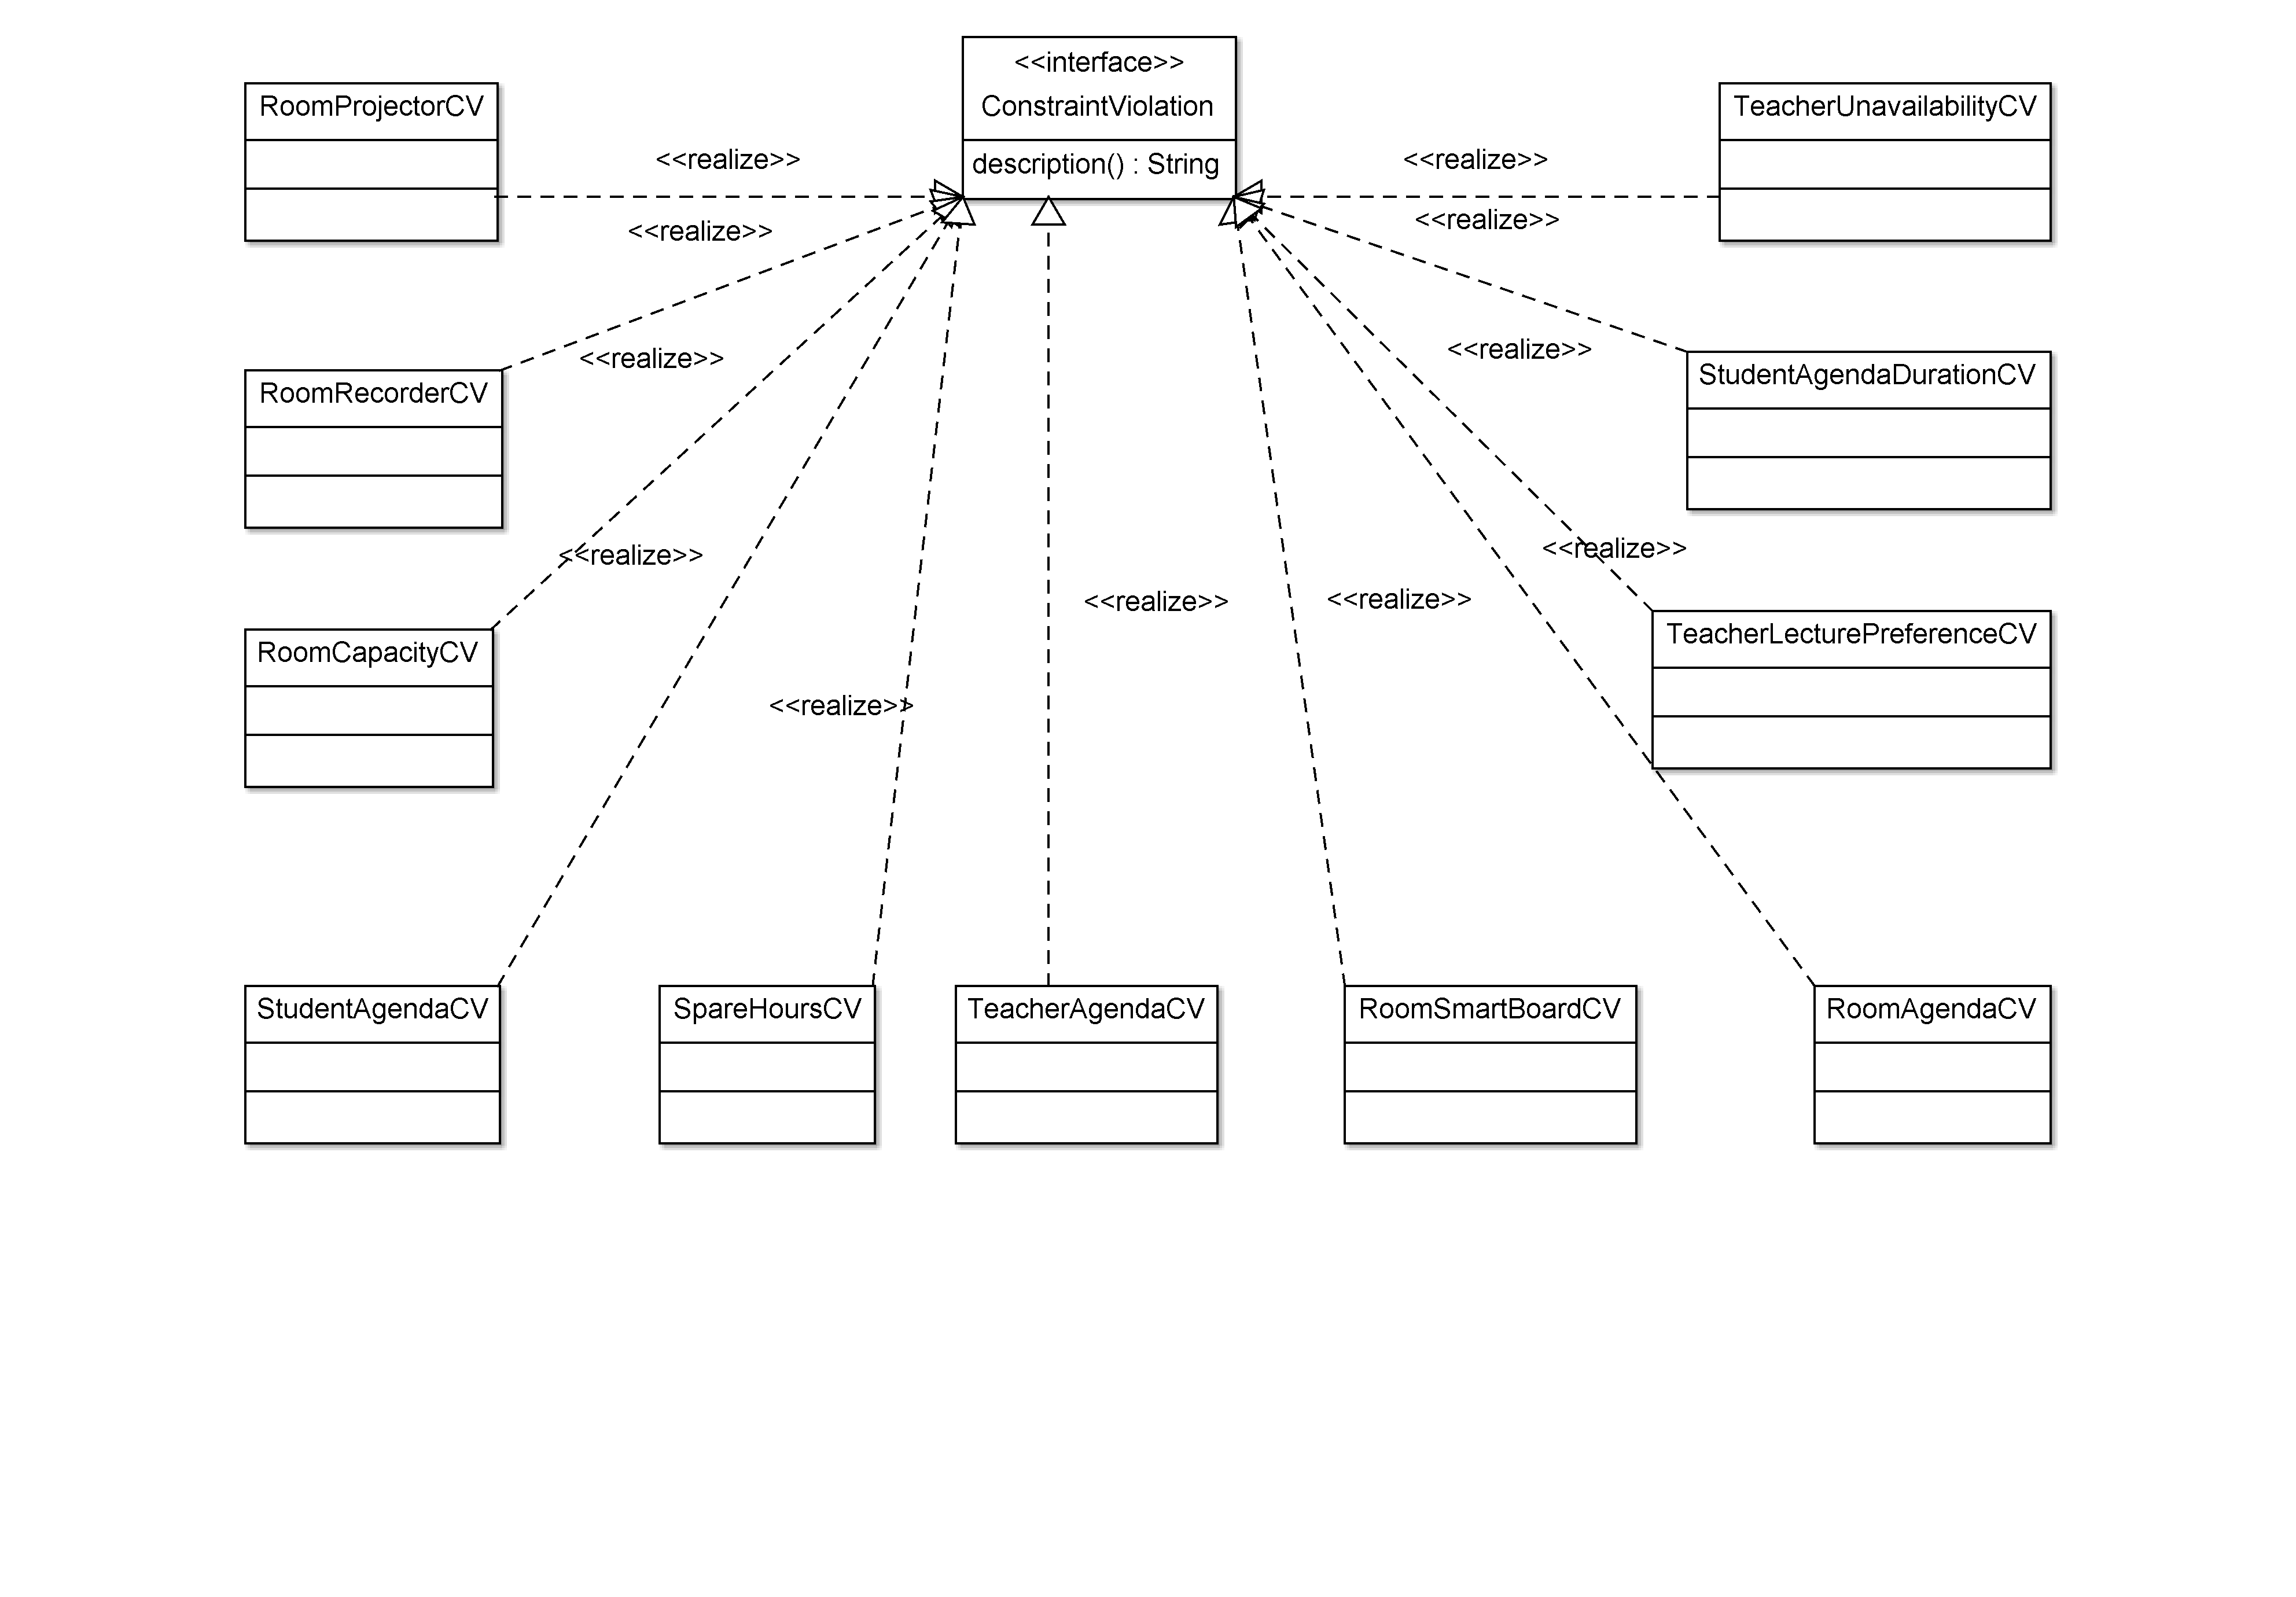
\includegraphics[scale=0.13]{img/constraintviolations}
	\caption{UML klassediagram van de verschillende ConstraintViolations}
	\label{fig:constraintviolations}
\end{figure}

\section{Algoritmes}
\label{sec:algorithms}
\subsection{Scheduling}
\label{subsec:scheduling}
Het huidige plan is om gebruik te maken van de Java Library 'Optaplanner'

\backmatter
	\nocite{*}
	\printbibliography

\end{document}